\section{Preliminares}\label{sec:prelim}

%% Agregar algo de firmas criptográficas.

En esta sección se presenta una breve descripción de los conceptos fundamentales
más importantes para hacer posible la comprensión y discusión sobre las
contribuciones de este trabajo.

\subsection{Sistemas distribuídos: donde todo comenzó}

La computación distribuída nació a fines de la década de 1970 cuando investigadores y profesionales
comenzaron a tener en cuenta las características intrínsecas de los sistemas distribuídos físicamente.
El campo luego emergió como un área de investigación especializada distinta al de redes, al de sistemas
operativos, y al de computación paralela.~\cite{raynal.dist.systems}

La computación distribuída surge cuando se tiene que resolver un problema en términos de entidades
distribuídas (usualmente llamadas procesos, nodos, actores, agentes, pares, etc) en donde cada
entidad tiene conocimiento parcial sobre los diversos parámetros involucrados en el problema que
se tiene que resolver. 
Es clave notar que el hecho de que las entidades (y la información que consume cada una de ellas)
estén distribuídas no es una propiedad que se encuentre bajo el control de los programadores, sino 
que es una imposición dada por las características propias del problema. En la 
Figura ~\ref{fig:distributed-systems} se expresa esto mediante un punto de vista
de la arquitectura del sistema, en donde cada par $(p_i, in_i)$ denota una entidad informática $p_i$ y su
entrada asociada $in_i$.

\begin{figure}
  \centering
  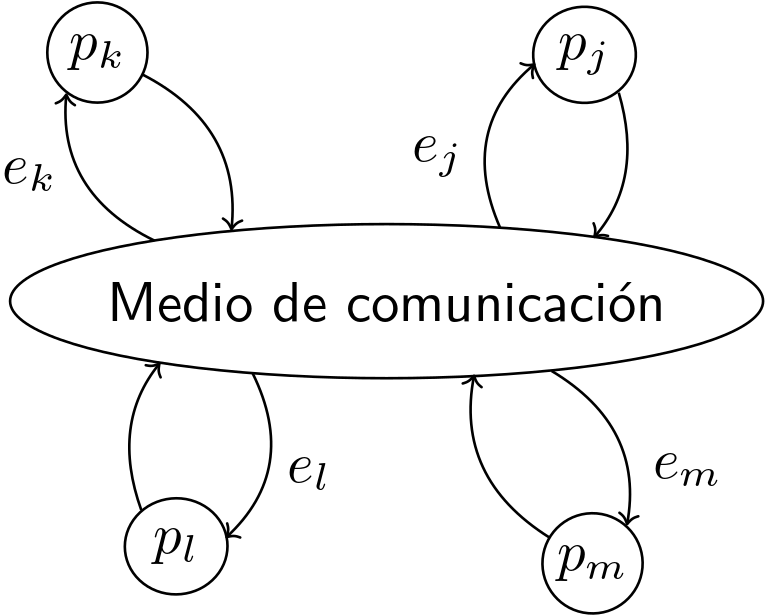
\includegraphics[scale=0.5]{figures/distributed-systems.png}
  \caption{Estructura básica de la computación distribuída}
  \label{fig:distributed-systems}
\end{figure}


Como se ilustra en la Figura ~\ref{fig:distributed-systems}, un sistema distribuído está hecho de una
colección de unidades de computación (llamadas también unidades informáticas) distribuídas, cada una
abstraída a través de la noción de un proceso, interconectada a través de un medio de comunicación.
Se asume que los procesos cooperan por un objetivo común, lo cual significa que intercambian
información de una manera u otra. Es interesante notar que el hecho de que las entidades
cooperen no significa la asumción de que todas las entidades se comportarán de la forma
acordada, ya sea por un error (por ejemplo, en la programación o en una red) o por un compartamiento
malintencionado. Se volverá a este punto en la sección ~\ref{subsubsec:consensus}.

% Two main process failures models are considered in this book:
% • Crash failures. A process commits a crash failure when it prematurely stops its execution. Until
% it crashes (if it ever crashes), a process correctly executes its local algorithm.
% • Byzantine failures. A process commits a Byzantine failure when it does not follow the behav-
% ior assigned to it by its local algorithm. This kind of failure is also called arbitrary failure
% (sometimes known as malicious when the failure is intentional). Let us notice that crash failures
% (which are an unexpected definitive halt) are a proper subset of Byzantine failures.
% A simple example of a Byzantine failure is the the following: while it is assumed to send the
% same value to all processes, a process sends different values to different subsets of processes,
% and no value at all to other processes. This is a typical Byzantine behavior. Moreover, Byzantine
% processes can collude to foil the processes that are not Byzantine.
% From a terminology point of view, let us consider an execution E (an execution is also called a
% run). The processes that commit failures are said to be faulty in E. The other processes are said to
% be correct or non-faulty in E. It is not known in advance if a given process is correct or faulty, this is
% specific to each execution.
% Given a process failure model, the model parameter t is used to denote the maximal number of
% processes that can be faulty in an execution.

% Fuente: Fault-Tolerant Message-Passing Distributed Systems An Algorithmic Approach

\subsection{Criptografía}

\subsection{Los orígenes de la blockchain}
% Fuente: Mastering Bitcoin. Programming the open blockchain.
Las blockchains tomaron popularidad con la invención de Bitcoin en 2008, luego de la publicación
de un artículo llamado \textit{Bitcoin: A Peer-to-Peer
Electronic Cash System}\footnote{Bitcoin: un sistema de dinero electrónico de par a par.}, escrito
bajo el pseudónimo de Satoshi Nakamoto.
Nakamoto combinó diversas invenciones previas como
\textit{b-money}~\cite{b.money} y \textit{HashCash}~\cite{hashcash} para crear un sistema de dinero electrónico completamente
descentralizado que, justamente, no necesita confiar en ninguna autoridad central para la emisión de monedas,
o la liquidación o validación de las transacciones. 
La innovación clave en Bitcoin fue el uso de un sistema de cómputo distribuído que lleva
a cabo una elección global de las nuevas transacciones cada 10 minutos, permitiendo
a la red descentralizada llegar a un consenso sobre el estado de las mismas. Estas transacciones
se guardan empaquetadas como bloques en una bitácora distribuída pública conocida como blockchain.~\cite{mastering.bitcoin}
%
Se dice que estas transacciones se encuentran totalmente ordenadas porque es posible determinar para
dos transacciones cualesquieras en la blockchain cuál de ellas ocurrió antes.

%Esto resolvió de forma elegante el problema del doble gasto,
%en el cual una misma unidad de moneda se utiliza dos veces. Previamente, el problema del doble gasto fue
%una debilidad de los sistemas de moneda digital que fue abordado mediante servidores de información centrales.

Bitcoin es una colección de conceptos y tecnologías que forman las bases de un ecosistema de dinero
digital.
%
Si bien la noción de bitcoin como criptomoneda no es imprescindible para la comprensión de las
contribuciones de este trabajo, es el primer caso de uso que da particular importancia a la blockchain
como tal y a su rendimiento. Por este motivo se considera pertinente presentar un breve resumen sobre
su funcionamiento.

\subsubsection{Funcionamiento de bitcoin}

Las unidades de moneda llamadas bitcoins son usadas para almacenar y transmitir valor a través
de los participantes de la red de bitcoin. Los usuarios se comunican entre ellos usando un protocolo 
específico principalmente mediante internet. La pila del
protocolo bitcoin, disponible como software de código abierto, se puede correr en una amplia gama de
dispositivos, incluyendo computadoras portátiles y teléfonos inteligentes, haciéndolo una tecnología
de fácil acceso.

Los usuarios pueden transferir bitcoins en la red y hacer básicamente cualquier operación que puede ser
realizada con monedas tradicionales: comprar y vender bienes, enviar dinero a personas u
organizaciones, o extender créditos. Los bitcoins también pueden ser vendidos, comprados, o intercambiados por
otras monedas en casas de cambio especializadas.

A diferencia de las monedas tradicionales, los bitcoins son completamente virtuales. No hay monedas
físicas e incluso no existen monedas en sí. Las monedas se representan en transacciones que transfieren
valor desde el remitente hacia el destinatario. Los usuarios de bitcoin poseen claves criptográficas
que permiten probar la propiedad de los bitcoins en la red. Con estas claves se pueden firmar las
transacciones para desbloquear el valor y utilizarlo transfiriéndolo a un nuevo dueño. 
%Las claves
%son a menudo guardadas en billeteras digitales en las computadoras o celulares de los usuarios. La
%posesión de una clave que puede firmar una transacción es el único prerequisito para utilizar bitcoin,
%poniendo el control enteramente en manos de cada usuario.

Bitcoin es un sistema distribuído de par a par. Como tal no tiene un servidor central o un punto de control.
Los bitcoins son creados a través de un proceso llamado \textit{minería}, el cual involucra una competencia
para encontrar solución a un problema matemático mientras se procesan las transacciones de bitcoin.
Cualquier participante de la red (es decir, cualquiera quien use un dispositivo que corre la pila
completa de protocolo de bitcoin) puede operar como minero, usando el poder de procesamiento de su
computadora para verificar y guardar transacciones. Cada 10 minutos, en promedio, alguien logra validar
las transacciones de los últimos 10 minutos y es compensando con bitcoin nuevo. Esencialmente, la minería
de bitcoins descentraliza la emisión de moneda y las funciones de compensación de un banco central, evitando
la necesidad del mismo.

El protocolo de bitcoin incluye algoritmos nativos que regulan las funciones de minería a lo largo de la
red. La dificultad de la tarea de procesamiento que los mineros deben realizar se ajusta dinámicamente
de modo que, en promedio, alguien tiene éxito cada 10 minutos sin importar la cantidad de mineros (y
de poder de cómputo) existente en un momento dado. El protocolo además disminuye a la mitad el ratio de creación
de bitcoins cada 4 años, y limita el número total de bitcoins que serán creados a un número fijo de
aproximadamente 21 millones de bitcoins.

%El resultado es que el número de bitcoins en circulación
%sigue una curva predecible fácilmente que llega a 21 millones para el 2140. Debido a la disminución de
%emisión de bitcoins, a largo plazo, el bitcoin es deflacionario. Incluso más, bitcoin no puede sufrir
%inflación por "imprimir" más dinero más allá de ratio esperado. 

%Detrás de escena, bitcoin es el nombre de un protocolo, una red de pares, y una innovación de
%computación distribuída.
Bitcoin representa la culminación de décadas de investigación en criptografía
y sistemas distribuídos, e incluye 4 innovaciones claves funcionando juntas:
\begin{itemize}
  \item Una red de par a par descentralizada (el protocolo de bitcoin).
  \item Una bitácora distribuída pública de transacciones organizadas en bloques (la blockchain).
  \item Un conjunto de reglas para la validación independiente de transacciones y la emisión de monedas (reglas de consenso).
  \item Un mecanismo para lograr un consenso global descentralizado en la blockchain (algoritmo de prueba de trabajo).
\end{itemize}

\subsubsection{La forma de la blockchain}

La blockchain es la bitácora pública de bitcoin, un registro ordenado y con fecha y hora de las transacciones.
Cada nodo completo en la red de bitcoin guarda independientemente una blockchain que contiene solo
bloques validados por ese nodo. Cuando cierta cantidad de nodos tienen los mismos bloques en su propia blockchain
se dice que llegaron a un consenso. 
%The validation rules these nodes follow to maintain consensus are
%called consensus rules. This section describes many of the consensus rules used by Bitcoin Core.

La Figura \ref{fig:blockchain} muestra una versión simplificada de una blockchain. En la sección de datos de un bloque
se agrupan y alojan una o más transacciones nuevas. Copias de cada transacción se hashean, los hashes luego
se emparejan, se hashean, se emparejan de nuevo, y se hashean hasta que queda un único hash: la raíz de un
\textit{merkle tree}~\cite{merkle.tree}. 

\begin{figure}[h]
  \centering
  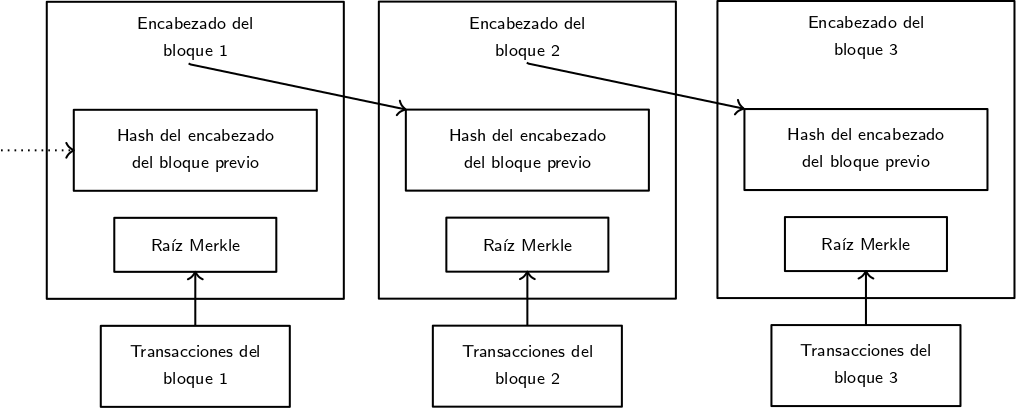
\includegraphics[scale=0.4]{figures/blockchain.png}
  \caption{Versión simplificada de la blockchain}
  \label{fig:blockchain}
\end{figure}


En la Figura \ref{fig:merkle-tree} se muestra un ejemplo de este tipo de árboles.
La raíz del merkle tree se aloja en el encabezado del bloque. Cada bloque además contiene el hash del encabezado
del bloque anterior, encadenándolos. Esto asegura que una transacción no pueda modificarse sin modificar el bloque
que la contiene y todos los bloques siguientes.~\cite{bitcoin}

\begin{figure}[h]
  \centering
  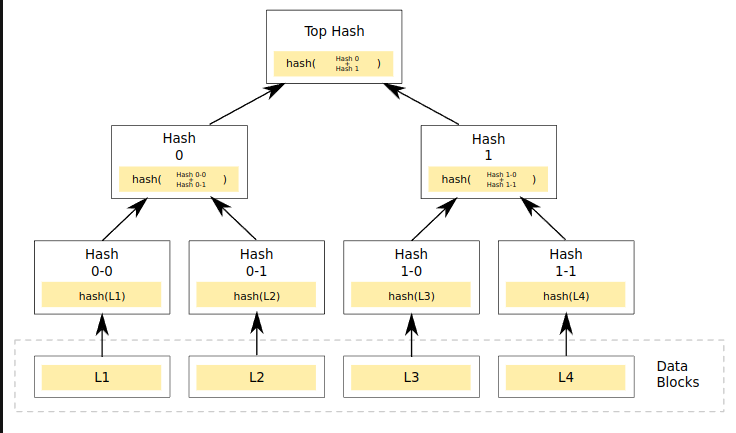
\includegraphics[scale=0.4]{figures/merkle-tree.png}
  \caption{Merkle tree}
  \label{fig:merkle-tree}
\end{figure}

%Las transacciones también están encadenadas. Es decir, cada transacción gasta los \textit{satoshis}\footnote{
%Satoshi es la unidad mínima de Bitcoin, llamada así por el pseudónimo de su creador, Satoshi Nakamoto. Un bitcoin
%es equivalente a 100 millones de Satoshis.} previamente recibidos en una o más transacciones previas, por lo
%que la entrada de una transacción es la salida de una transacción previa.

% Fuente: https://developer.bitcoin.org/devguide/block_chain.html

%\subsection{Blockchain actuales}

\subsection{Algoritmos de consenso}\label{subsubsec:consensus}
El problema de consenso es uno de los más celebrados en los sistemas de computación distribuída tolerante a fallas.
%
Abstrae diversos problemas en donde, de una manera u otra, los procesos deben ponerse de acuerdo.
%

Los problemas de consenso requieren acuerdo entre un número de procesos para determinar un valor particular.
%
Algunos de los procesos pueden fallar o ser no confiables de diversas maneras, por lo que los protocolos de
consenso deben ser resilientes a fallas.
%
Los procesos deben de alguna forma establecer sus valores candidatos, comunicándose entre ellos, y
poniéndose de acuerdo en un valor específico.
%
Los protocolos que resuelven el problema de consenso son diseñados para lidiar con un número limitado de procesos
que fallan.
%
Estos protoclos deben satisfacer un número de requerimientos para ser utilizados.
%
A lo largo de la historia se han desarrollado distintos algoritmos de consenso, que funcionan bajo diferentes
escenarios (cantidad de nodos, cantidad de nodos que pueden fallar, formas en las que pueden fallar, etc.)

%

Si bien a lo largo de este trabajo no se entrará en detalles sobre ningún algoritmo de consenso en particular,
es pertienente discutir conceptos y nomenclatura básica.

\subsubsection{El problema de los generales bizantinos}

Los sistemas de computación confiables deben lidiar con componentes que, por mal funcionamiento,
dan información conflictiva a diferentes partes del sistema. La situación puede ser exrepsada abstractamente
en términos de un grupo de generales de la armada bizantina que acampan con sus tropas alrededor de una
ciudad enemiga. Comunicándose solo a través de mensajeros, los generales deben ponerse de acuerdo en una plan
de batalla común. Sin embargo, uno o más de ellos pueden ser traidores, quienes tratarán de confundir a los
otros. El problema es encontrar un algoritmo que asegure que los generales leales lleguen a un acuerdo.
Está demostrado que, usando solo mensajes orales, este problema es resoluble si y solo si más de dos tercios
de los generales son leales.
La habilidad de tolerar máquinas que fallan de formas arbritarias, incluyendo aquellas maliciosas,
es conocida como tolerancia a fallas bizantinas (BFT por sus siglas en inglés). Si bien la teoría de
BFT es de décadas pasadas, las implementaciones de software se han vuelto populares recientemente,
debido al amplio éxito de tecnologías blockchains como Bitcoin y Ethereum.

% Fuente: [10] Lamport, L., Shostak, R., and Marshall, P. The byzantine generals problem.


\subsection{Setchain}~\label{sec:setchain}

\setchain~\cite{Capretto.2022.Setchain} es un tipo de datos concurrente y distribuído que implementa
conjuntos distribuídos de solo crecimiento, con barreras de sincronización (llamadas épocas), y tolerante
a comportamiento bizantinos.
%
Las barreras imponen un orden entre elementos pertenecientes a diferentes épocas pero no entre elementos
de la misma época.
%
Por lo tanto, \setchain relaja el requerimiento de orden total impuesto por las blockchains y, en consecuencia,
puede lograr mayor rendimiento y escalabilidad.

\subsubsection{La interfaz de Setchain}
Sea \(U\) un conjunto de elementos que los procesos clientes pueden inyectar en la \setchain.
%
Sea \isValidElement\ una función que los nodos pueden usar para validar elementos en \(U\)
localmente.
%
Una \setchain es una estructura de datos distribuída donde una colleción de nodos servidores
mantienen:
\begin{itemize}
  \item un conjunto $\THESET \subseteq U$ de elementos agregados;
  \item un número natural $\EPOCH \in \mathds{N}$;
  \item una función $\HISTORY : [1..\EPOCH] \rightarrow \mathcal{P}(U)$\footnote{$\mathcal{P}(U)$ denota el conjunto potencia
  de $U$} que describe los conjuntos de elementos que fueron estampados con un número de época.
\end{itemize}

%
%Los nodos servidores soportan dos operaciones: \Add y \Get.
%
%La operación \Add agrega un elemento, mientras que la operación \Get retorna la terna (\THESET,\HISTORY,\EPOCH) mantenida
% por el nodo.

% %

%Se usará notación de punto para invocar estas operaciones. Sea $v$ un nodo servidor, y $e$ un elemento:
%se notará $v.\Add(e)$ para solicitarle añadir el elemento $e$ al nodo $v$, y $v.\Get$ para pedirle al nodo $v$
%que retorne la terna en cuestión.

Cada nodo servidor $v$ soporta dos operaciones, disponibles para todos los procesos clientes:
\begin{itemize}
  \item $v.\Add(e)$: solicita agregar el elemento $e$ a $\THESET$.
  \item $v.\Get()$: retorna los valores de $\THESET $, $\HISTORY $,
    and $\EPOCH $, según $v$.
\end{itemize}
  
Cuando se impone una nueva barrera de sincronización, los nodos que mantinen la \setchain colaborativamente
deciden cuáles elementos añadidos son estampados con la época actual, y se incrementa el número de época.
%
Estos eventos se llaman \textit{incrementos de época}.
%
Se asume que las barreras de sincronización se lanzan periódicamente.
%
Un flujo de trabajo típico desde el punto de vista del cliente es como sigue: un cliente invoca $\Add(e)$ en
uno (o más) servidores para insertar un nuevo elemento válido $e$ en la \setchain.
% 
El elemento $e$ será propagado hacia los servidores, y cuando un incremento de época ocurra, los servidores
intentarán incluirlo en la nueva época.
%
Después de esperar cierto tiempo, el cliente invoca \Get en uno (o más) servidores para chequear que el
elemento fue efectivamente agregado y estampado con una época.

\subsubsection{Propiedades}
Para asegurar correctitud, las implementaciones de \setchain deben satisfacer ciertas propiedades que
proveen garantías eventuales para elementos añadidos y garantía de consistencia entre los servidores
correctos.
%
Estas propiedades razonan sobre los servidores correctos, dado que los servidores bizantinos no proveen
ninguna garantía.

\begin{itemize}
  \item Cada elemento válido agregado por un servidor correcto eventualmente es retornado en
  todas las futuras invocaciones a \Get hechas sobre servidores correctos.
  \item Todos los elementos válidos agregados en un servidor corrector deben eventualmente ser
  estampados con un número de época en todos los servidores correctos.
  \item Una vez que un elemento es estampado con una época, no puede ser des-estampado, ni puede
  ser estampado con otro número de época.
  \item Dos servidores correctos cualesquieras están se acuerdo en el contenido de todas las épocas
  que hayan sido computadas~\footnote{No todos los servidores correctos procesan los incrementos de
  época simultáneamente, dado que algunos pueden estar más retrazados que otros.}.
  \item Cada elemento que se estampa con una época proviene del resultado de un cliente añadiendo
  el elemento.
\end{itemize}
% \gabina{Epoch proofs are part of the epoch but are not coming directly from the result of a client adding element.}

\subsection{Tendermint}\label{sec:tendermint}
Tendermint es un motor de replicación de máquinas de estado que tolera fallas bizantinas.
%
Fue uno de los primeros sistemas en adaptar protocolos de consenso clásicos tolerantes a fallas bizantinas
al paradigma de blockchain.
%
Es decir, donde el consenso se ejecuta sobre lotes de transacciones vinculados mediante
hashes criptográficos (usualmente llamados bloques) en una red pública y abierta.

%

Tendermint funciona como una capa intermedia de blockchain que soporta la replicación de aplicaciones arbitrarias,
escritas en cualquier lenguaje de programación~\cite{tendermint.design}.
%
En la Figura~\ref{fig:replication} se muestra un esquema general de la arquitectura de la replicación de máquinas de
estado.
%
Las transacciones se reciben desde el cliente, quien se comunica, mediante una API, con una (o más) de las máquinas
en la red.
%
Estas transacciones pasan a través del protocolo de consenso, quien es el encargado de ordernar dichas
transacciones en bloques, mediante una serie de pasos que involucra comunicación entre todas las máquinas
(señalizada en la figura con líneas punteadas).
%
Una vez ordenadas, las transacciones son ejecutadas en cada una de las máquinas, modificando el estado
de cada una de ellas.
%
De esta forma, se replican lotes de transacciones enviadas por los distintos clientes, que son ejecutadas en el mismo
orden en cada una de las máquinas en la red, resultando en un mismo estado a lo largo de múltiples máquinas.
%
Las figuras azules representan máquinas.
%
Las líneas punteadas representan la comunicación entre máquinas para llevar a cabo el protocolo de consenso para ordernar
transacciones.

\begin{figure}
  \centering
  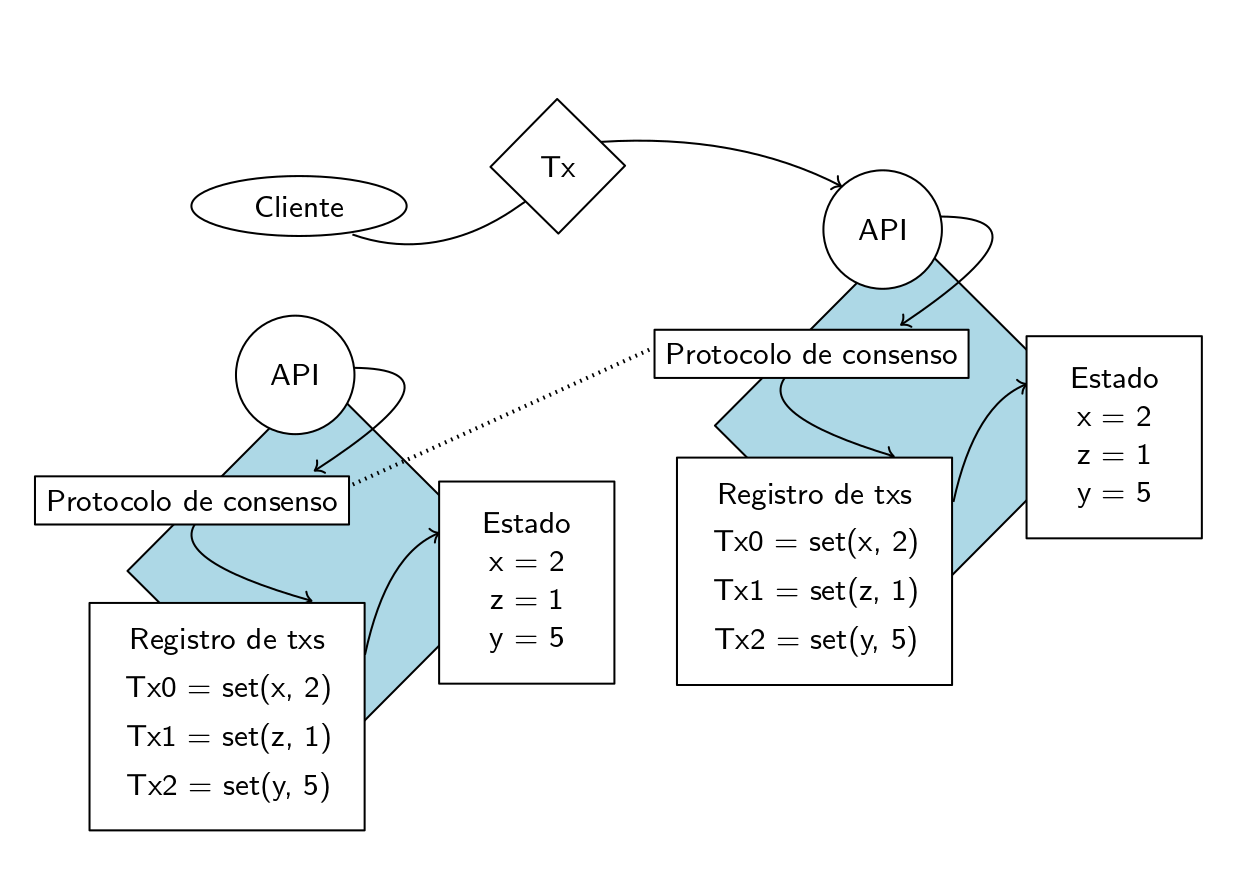
\includegraphics[scale=0.3]{figures/state-machine-replication.png}
  \caption{Esquema simplificado de la replicación de máquinas de estado.}
  \label{fig:replication}
\end{figure}

\subsubsection{Arquitectura de capas de Tendermint}\label{subsec:layers}

La Figura~\ref{fig:tendermint-architecture} presenta la estructura básica de Tendermint como un sistema de capas.
La subcapa inferior se encarga de la comunicación entre pares, y provee comunicación para los principales
módulos de la blockchain. Éstos son los módulos que se presentan en la capa inmediata superior: mempool, consenso,
evidencia, sincronización rápida, y sincronización de estado. Para el presente trabajo, solo serán pertinentes los
módulos de mempool y de consenso.

Un cliente interactúa con el sistema mediante RPC al enviar transacciones
que (en caso de ser válidas) son añadidas al módulo de mempool. El cliente en general
recibe respuestas generadas por el módulo de consenso.
El módulo de consenso se encarga de ordenar e intermediar la ejecución de las transacciones, por medio de la
interfaz de aplicación.

\begin{figure}
  \centering
  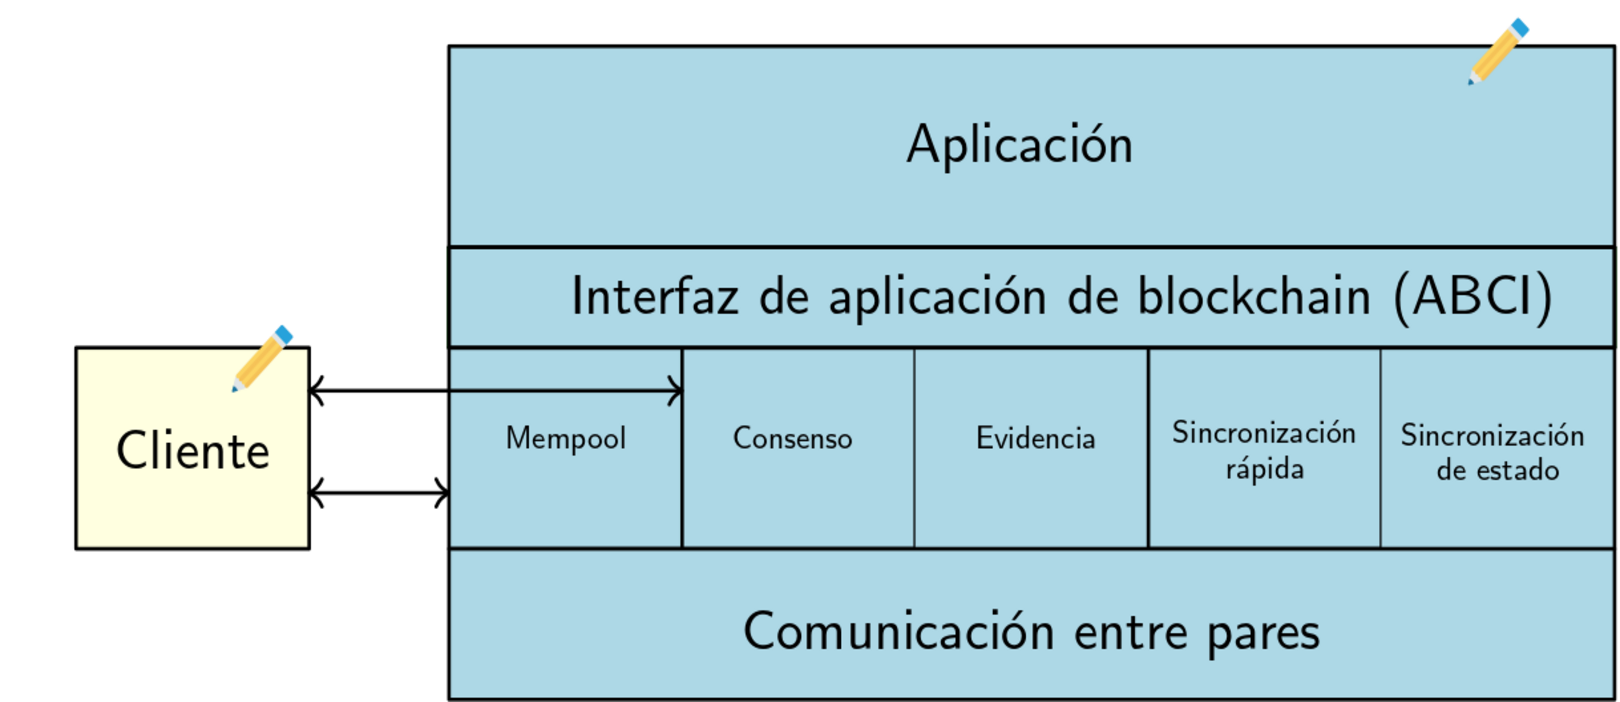
\includegraphics[scale=0.2]{figures/tendermint-layers.png}
  \caption{Arquitectura de capas de Tendermint.}
  \label{fig:tendermint-architecture}
\end{figure}

% %
Tendermint consiste de dos componentes técnicos principales: un motor de consenso de blockchain, y una interfaz
de aplicación genérica.
%
El motor de consenso, llamado \textit{Tendermint Core}, asegura que las mismas transacciones sean registradas en cada
máquinas en el mismo orden.
%
La interfaz de aplicación, llamada \textit{interfaz de aplicación de blockchain} (IABC)\footnote{Proveniente de \textit{Application
BlockChain Interface} (ABCI) en inglés.}, habilita que las transacciones
sean procesadas en cualquier lenguaje de programación.

\subsubsection{Application BlockChain Interface}\label{subsec:abci}
La interfaz de aplicación de blockchain es la interfaz entre el Tendermint Core y la aplicación replicada.
%
Un nodo de Tendermint mantiene tres conexiones ABCI con la aplicación replicada.
%
La \textit{conexión de consenso} se utiliza solo cuando se hace \textit{commit} sobre un nuevo bloque,
y comunica toda la información del bloque mediante una serie de peticiones: 
\BeginBlock, [\DeliverTx, ...], \EndBlock, \Commit.
%
Esto significa que, cuando un bloque es acordado meidante consenso, Tendermint envía una petición \BeginBlock
seguida por una lista de peticiones \DeliverTx (una por cada transacción en el bloque), que finalizan con las
peticiones \EndBlock y \Commit, en ese orden.

%

La \textit{conexión de mempool} es usada por el protocolo de reserva de transacciones \footnote{\textit{Transaction pool protocol}
en inglés.} para validar las transacciones enviadas por los clientes en relación al estado de la aplicación.
%
Esta conexión solo admite peticiones \CheckTx. Las transacciones se chequean (mediante \CheckTx) en el mismo orden
en que fueron recibidas por el nodo validador\footnote{Los nodos validadores son responsables de hacer commit sobre nuevos
bloques en la blockchain. Estos validadores participan en el protocolo de consenso mediante la difusión de votos, los
cuales contienen firmas criptográficas generadas por las claves privadas de cada validador.}.
%
Si \CheckTx retorna \textit{OK}, la transacción se mantiene en memoria y se retransmite a otros pares en el mismo orden
en que fue recibida.
%
En caso contrario, se descarta.
%
Es parte de la lógica de la aplicación definir cuándo una transacción es válida o no, e incluso la validación es opcional.
%
De esta manera, queda claro que Tendermint es agnóstico de la semántica de las transacciones.

%

La \textit{conexión de consulta} permite recuperar información de la instancia local de la aplicación, usada
por distintos módulos de Tendermint (tales como el módulo de filtrado de pares).
%
Se utiliza para consultar la aplicación sin forzar consenso.
%
Se expone mediante el servidor RPC\footnote{\textit{Remote Procedure Call} o llamada a procedimiento
remoto en español.} del Tendermint Core, de modo que los clientes pueden
consultar el estado de la aplicación sin exponer un servidor de la aplicación en sí mismo. 

La Figura~\ref{fig:abci_flow} muestra el flujo de mensajes mediante las conexiones de consenso y de mempool.

\begin{figure}
  \centering
  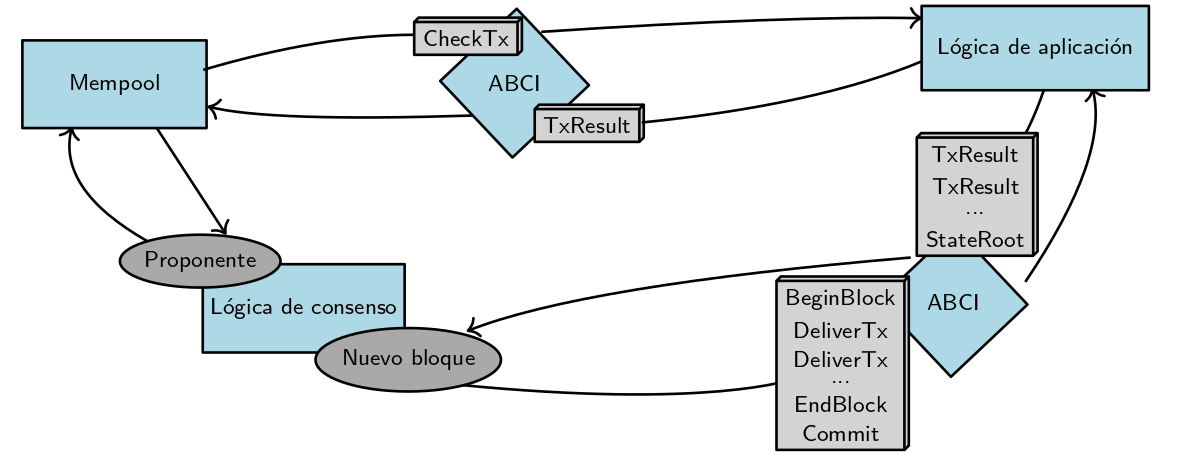
\includegraphics[scale=0.35]{figures/abci_msg_flow.png}
  \caption{Flujo de mensajes mediante la ABCI.}
  \label{fig:abci_flow}
\end{figure}

%%% Local Variables:
%%% TeX-master: "article.tex"
%%% TeX-PDF-mode: t
%%% End:
